\chapter[Background information]{Background information} \label{ch:background}

\section{Chapter 2: transportation and land use, land registration in Canada and Teranet} \label{sec:chapter_2_intro}

This chapter discusses the complex interaction of land use and transportation, provides a brief overview of the history of development of land use-transportation (LUT) models, presents some legal and historical background for Teranet's dataset of real estate transactions and finishes with discussing challenges of working with Teranet's data and the proposed solution.

\section{Land Use and Transport (LUT) models} \label{sec:evolution_of_models_of_urban_systems}

\subsection{Complexity of urban systems and "wicked" problems} \label{subsec:complexity_and_wicked_problems}

In her famous 1961 book, Jane Jacobs\cite{Jacobs1961} described a city as "a problem in organized complexity";
since then, many other researchers have remarked that urban systems exhibit complex behaviour\cite{Batty2008, Bettencourt2013}.
Complexity of a system can be defined as a state or quality of being intricate or complicated.
For a system to be complex is not necessarily the same as to be complicated;
complex systems can be simple, i.e.\ governed by a single equation.
Complexity of a system has to do with the intrinsic ability of a system to surprise us with its behaviour;
that the system is hard to understand, despite the mechanics of it being relatively simple.

In 1973, a little over a decade after Jacobs, Rittel and Webber\cite{Rittel1973} presented a path-breaking conceptualization;
this conceptualization characterized urban planning problems as "wicked" problems: problems which cannot be definitively described and for which it makes no sense to talk of "optimal solutions".
In their paper, Rittel and Webber stated that such "wicked" problems are never "solved", and that the focus instead becomes on iteratively "re-solving" the problems over and over.
More than 40 years after their original publication, Rittel and Webber's ideas remain relevant to the policy sciences today: there is an intense interest in the nature of "wicked" problems and the complex tasks of identifying their scope, viable responses, and appropriate mechanisms and pathways to improvement\cite{Crowley2017}.
Interaction between land use and transportation systems which is discussed in the following section presents a prime example of urban complexities and "wicked" problems.

\subsection{Transportation-land use cycle} \label{subsec:transportation_land_use_cycle}

Among the reasons why transportation and land use interaction is "wicked" are such aspects as pluralism of expectations among stakeholders, institutional complexity in policy making, and scientific uncertainty\cite{Noto2015}.
There is a fundamental link between transportation and urban form: the nature of development of urban areas directly determines such aspects as travel needs, viability of alternative modes, relative accessibility, and other important characteristics of an urban transportation system.
Transportation, in turn, influences land development and location choices of people and firms\cite{Miller1999}.
This relationship is sometimes referred to as the transportation-land use "link" or "cycle", emphasising a feedback relationship\cite{Kelly}.

Figure~\ref{fig:idealized_integrated_urban_model} illustrates the complex interactions between land use and transportation system as summarized by Miller\cite{Miller2018a}.

\begin{figure}[hbt!]
    \centering
    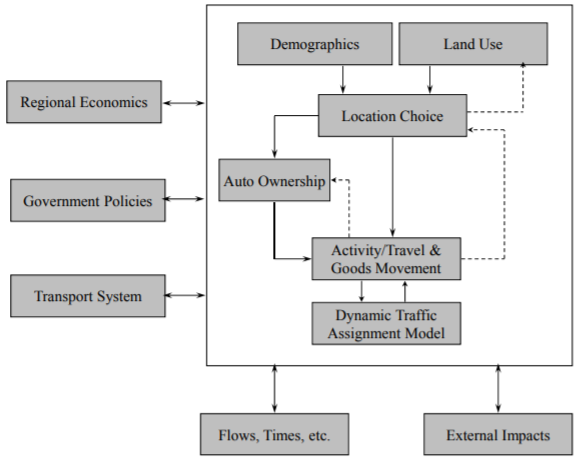
\includegraphics[width=0.7\linewidth,trim=0 0 0 0,clip]{miller_idealized_urban_model.png}
    \caption{An Idealized Integrated Urban Model System\cite{Miller2018a}.}
    \label{fig:idealized_integrated_urban_model}
\end{figure}

\subsection{Accessibility as a measure of land use-transportation relationship} \label{subsec:accessibility}

While transportation research started as an isolated field focusing on mobility, researchers recognized that trips are made to access particular destinations\cite{VanLierop2017}.
A concept of accessibility, understood as the ease of reaching rather than simply the ease of moving\cite{Preston2007}, was developed to take into account the location of urban opportunities.
Accessibility is the mediating factor between the location of activities and demand for travel and is discussed further in section~\ref{subsec:accessibility} of the following chapter.

LUT models (discussed in section~\ref{subsec:transportation_land_use_interaction}) operationalize the transportation-land use relationship by incorporating measures of accessibility with the process of locating activities, typically assuming that households wish to locate in areas with higher accessibility to employment, shopping, or entertainment opportunities.
Similarly, firms are assumed to locate in areas with higher accessibility to labour markets.
Land use component is usually integrated into the accessibility measure through congested network travel times.
However, when studying the relationship between transportation facilities and property values, results may vary based on whether travel time or travel distance is used as a measure of accessibility\cite{Sherry1999}.

Accessibility measures the situation of a location relative to other activities or opportunities (work, shopping, etc.) distributed in space and can be an important determinant of price in LUT models where land and floor space markets are considered explicitly\cite{Iacono2008}.
When measuring changes in relative accessibility, it is usually approximated by some measure of access to the transportation network, such as travel time or distance.

Economic decisions made by the households and firms act as one of the links between the tranportation and land use systems.
When choosing a location, households and firms attempt to fulfill as many of their location preferences as possible while facing constraints.
One of the main constraints is the price or rent of the dwelling, related to the income of the household;
another important constraint is travel time, with suitable location being restricted by the travel times and transportation expenses\cite{Moeckel2017}.

\subsection{Models used for transportation and land use} \label{subsec:transportation_land_use_interaction}

Many different types of models are used in planning, such as demand forecasting models projecting traffic or ridership, or land use models projecting and distributing population and jobs within an area, as well as integrated land use-transportation models.
Integrated land use-transportation models combine travel demand forecasting and land use forecasting functions and recognize that the distribution of population and jobs depends, in part, on transportation accessibility.
The reverse is also true, and thus integrated models incorporate feedback relationship between transportation and land use, with economic decisions by households and firms acting as one of the links between the two systems\cite{Miller1999}.

Iacono et al.
\cite{Iacono2008} provide an overview of some of the most common frameworks of Land Use and Transport (LUT) models that have been used to model interaction between transportation and land use in urbanized regions.
Despite the difficulty of modelling of every relevant aspect of an urban region, a wide variety of models were produced dealing with the relationship between transportation network growth and changes in land use and the location of economic activity.
The frameworks can broadly be broken into two major approaches to modelling interactions between land use and transport:
\begin{itemize}
    \item "top-down" modeling frameworks, where interaction between transportation networks and location is specified as a set of aggregate relationships.
    These relationships are based on the behaviour of a representative individual, and are usually taken as a mean calculated from a representative sample of the population.
    These models include:
    \begin{itemize}
        \item aggregate models of spatial interaction
        \item econometric models
    \end{itemize}
    \item "bottom-up" microsimulation models, which cover a number of different approaches to representing the dynamics of land use change and travel behaviour through disaggregating the population and simulating the changes.
    These models include:
    \begin{itemize}
        \item activity-based travel models
        \item multi-agent models
        \item cell-based models
    \end{itemize}
\end{itemize}

\subsection{Evolution of LUT models} \label{subsec:evolution_of_lut_models}

The history of treating cities as systems via simulation models of transportation and land use dates back to 1950s when General System Theory and Cybernetics came to be applied in the softer social sciences\cite{Batty2008}.
Figure~\ref{fig:lut_model_evolution} provides the general overview of chronological development of LUT models summarized by Iacono\cite{Iacono2008}.

\begin{figure}[hbt!]
    \centering
    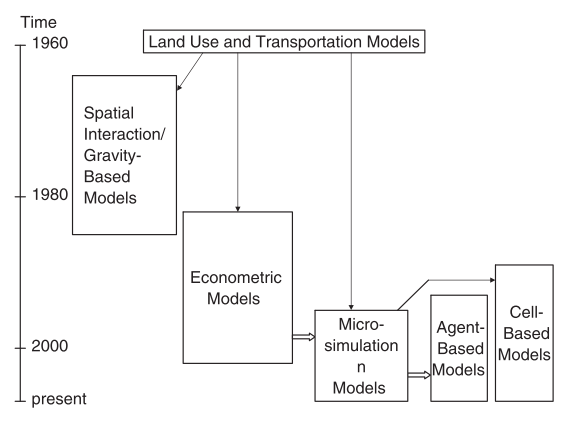
\includegraphics[width=0.7\linewidth,trim=0 0 0 0,clip]{lut_models_evolution.png}
    \caption{Chronological development of LUT models summarized by Iacono\cite{Iacono2008}.}
    \label{fig:lut_model_evolution}
\end{figure}

The first operational simulation model that truly integrated land use and transportation is considered to be A Model of Metropolis built in 1964 by Ira S. Lowry based on economic base theory for the Pittsburgh region\cite{Lowry1964}.
It was a highly aggregate model based on theories of spatial interaction, such as the gravity model that was popular in quantitative geography and transportation planning at the time\cite{Bouchard1965}.
Models based on spatial interaction framework continued to be developed through mid-1980s, until developments in random utility theory allowed researchers to describe choices among discrete alternatives, such as the choice of travel mode, and generate models based on the study of disaggregate behaviour\cite{Iacono2008}.

The modeling paradigm has changed fundamentally in the early 1990s along with advances in computing power and efficiency of data storage.
Urban systems used to be viewed as hierarchical and centrally organized equilibrium structures, or "top-down".
Instead, now they were considered to be structured from the "bottom-up", dynamically retaining their integrity through interactions of numerous microelements\cite{Batty2008}.
A new broad class of LUT models that could fall under the title of "microsimulation" began to be developed.
It included such classes of models as activity-based travel, cell-based models, and multi-agent models, and more recently comprehensive urban microsimulation models that fully reflect the dynamics of changes in the population and the urban environment\cite{Iacono2008}.

\subsection{ILUTE model system} \label{subsec:ilute}

The Integrated Land Use, Transportation, Environment (ILUTE) model system is an operational agent-based microsimulation model for greater Toronto-Hamilton area.
It uses disaggregate models of spatial socioeconomic processes to evolve the state of the greater Toronto\textendash Hamilton area from a known base case to a predicted end state in 1-year time steps.
The system state is defined in terms of the individual persons, households, dwelling units, firms, etc.
that collectively define the urban region being modeled\cite{Miller2011}.
ILUTE model simulates the evolution of an urban region's spatial form, demographics, travel behavior and economic structure over time.


The Housing Market Evolutionary System (HoMES) is the updated housing market module for the ILUTE model system.
HoMES is a disaggregate, agent-based microsimulation of the owner-occupied housing market that evolves the residential location of households over time and includes the endogenous supply of housing by type and location, as well as the endogenous determination of sales prices and rents.
An overview of the framework of housing market supply, demand and clearing mechanisms utilized in HoMES provided by Rosenfield et al.\cite{Rosenfield2013} is presented on figure~\ref{fig:homes_framework}

\begin{figure}[hbt!]
    \centering
    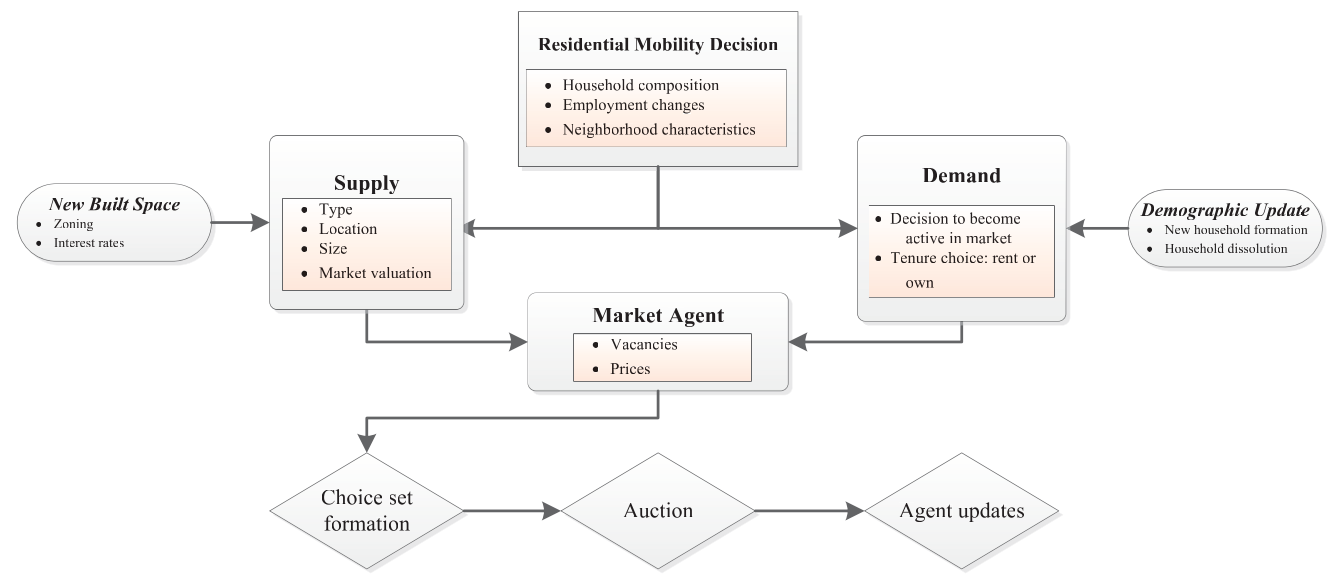
\includegraphics[width=0.99\linewidth,trim=0 0 0 0,clip]{homes_framework.png}
    \caption{Framework of housing market supply, demand and clearing mechanisms used in HoMES module of ILUTE, as summarized by Rosenfield et al.\cite{Rosenfield2013}.}
    \label{fig:homes_framework}
\end{figure}

%TODO transition to housing market data

\section{System of land registration in Canada, POLARIS and Teranet} \label{sec:system_of_land_registration_polaris_teranet}

\subsection{System of land registration in Canada} \label{subsec:land_reg_system_canada}

According to Chapter 6 of the International Comparative Legal Guide to Real Estate published by the Global Legal Group in 2015\cite{McKean2015}, all land owned in Canada is registered in a public land registry through either a registry system, a land titles system or a combination of both in the applicable province.
The registry system is a public record of documents evidencing transactions affecting land.
In the land titles system, the applicable provincial government determines the quality of the title, and essentially guarantees (within certain important statutory limits) the title to, and interests in, the property.
As of 2015, most common law provinces and territories were using the land titles system or were in the process of converting title from a registry system to a land titles system.

On the purchase and sale of real estate and land, ownership is generally transferred to the buyer when the deed or transfer is registered in the applicable land registry office.
An agreement of purchase and sale must be in writing to be enforceable.
A transfer of ownership is actualised by registering, either physically or electronically (depending on the applicable land registry system), a deed or transfer with the applicable land registry office or land registrar, copies of which can be obtained from the relevant registry office, often electronically.

\subsection{POLARIS: Land registration system of Ontario} \label{subsec:polaris}

Each province and territory in Canada has its own land registry system, whether it is a land titles system, a registry system or a combination of both, with each system having its own rules.
As of 2015, the Province of Ontario has largely converted from registry systems to a land titles system.

In 1985, the Government of Ontario initiated the Province of Ontario Land Registration Information System (POLARIS) pilot project for the purposes of records automation and the conversion from the Registry System to the Land Titles System.
The Land Registration Reform Act (Ontario)\cite{TheGovernmentofOntario1990} was introduced in 1990 to facilitate electronic search and registration of properties and the automation of paper-based records.

POLARIS was built by the Province to house and process electronic land records, which in turn lead to the creation of an extensive dataset of land registration records managed by Teranet Enterprises Inc.
Today, POLARIS is the search/registration and property maintenance system for all automated land records in Ontario.

\subsection{The Teranet-Ontario Partnership} \label{subsec:teranet_ontario}

In 1991, the Government of Ontario established a partnership with Teranet\cite{TeranetEnterprisesInc.2019}, a Toronto-based organization, founded the same year, which provides e-services to legal, real estate, government, financial, and healthcare markets.
The partnership was established to convert Ontario's land registration system to a more modernized electronic title system.
The project involved taking a 200-year-old paper-based system and creating a database with electronic records for more than five million parcels of land.

Teranet converted all qualified Registry properties in Ontario to the Land Titles system and automated existing paper Land Titles parcels.
As a result, 99.9\% of property in Ontario was parcelized and administered under the Land Titles system, which affords a property ownership guarantee by the province.
Teranet fully automated the conversion of millions of paper-based documents and records into the Ontario Electronic Land Registration System (ELRS).

In December 2010, the Government of Ontario extended its exclusive relationship with Teranet by 50 years.
Today, Teranet is the exclusive provider of Ontario's online property search and registration;
it developed, owns and operates the ELRS, and also provides online access to Ontario's Writs System.

\section{Challenges of using Teranet's data and the proposed solution} \label{sec:challenges}

This approach resembles the methodologies typically employed for data science projects, where the sequence of steps is iterated over, producing a more meaningful solution on each new iteration of the cycle, as defined by such process models as CRISP-DM\cite{Shearer2000}.
As an increasing amount of aspects of human life becomes digitalized, a wealth of new data is produced and can be used to model and analyze dynamics of urban systems\cite{Arribas-Bel2014, Chen2016}.
An example of such digitalization of human activity is the introduction of the Province of Ontario Land Registration Information System (POLARIS) in 1985 by the Government of Ontario\cite{TeranetEnterprisesInc.}.
This lead to the creation of an extensive dataset of real estate transactions by Teranet Enterprises Inc.
that offers a very fine resolution of housing market data across both time and space, but also presents challenges discussed in section~\ref{sec:challenges}.
To address these challenges, an efficient and modular Python workflow and a relational database for GTHA housing market are introduced with this master's thesis.
This makes data science methodologies a natural fit when trying to get a deeper understanding of the nature of "wicked" urban problems, such as the interaction between land development, urban form, and transportation.

\subsection{Data quality, skill requirements and lack of features} \label{subsec:challenges_quality_skills_features}

Teranet dataset presents an extensive historical record of real estate transactions recorded in the Province of Ontario since the beginning of XIX century.
However, when it comes to using new data sources in social studies, along with opportunities there are also challenges present.
For example, these data sources can have issues with the quality of the data, might require a specific set of skills to take advantage of these data sources, or might not be suitable for traditional methods meant for traditional data\cite{Arribas-Bel2014}, all of which are true in the case of Teranet's dataset.

On top of the issues with Teranet's data mentioned above, the most significant challenge lies in the amount of features provided for each record.
Despite capturing effectively the complete population of real estate transactions recorded in Ontario since 1985, the available version of the dataset includes no information describing anything about each transaction, other than its location in the form of address and coordinates, the registration date, and the consideration amount.
Since is no distinction being made between transactions recorded for residential, commercial, and industrial property types, transaction amounts can vary from several dollars to billions of dollars.
There are no attributes that would allow transactions to be filtered for meaningful analysis and modeling.

\subsection{Size of datasets, computational requirements and file formats} \label{subsec:challenges_size_and_formats}

To address this gap, additional attributes can be joined from various data sources, such as Census, TTS or land use data, based on spatial or temporal relationships.
However, Teranet's dataset has a number of records on the order of $10^6$.
Such data sources as Census tables have the number of fields on the order of $10^2$.
Overall, the number of attributes that could be joined between the various available data sources will probably be on the order of $10^3$.
This fact makes it increasingly impractical to store all the data in one table, due to the memory requirements for storage and processing.

In addition, datasets coming from different sources arrive in different file formats, such as text files, Excel spreadsheets, .csv files, or shapefiles.
Combined with the size of the datasets and the computational requirements of such processing techniques as spatial joins, the facts mentioned above make working with Teranet's difficult due to the hardware and special skill requirements.

\subsection{Complex spatial and temporal relationships between urban data sources} \label{subsec:complex_spatio-temporal_relationships_between_urban_data_sources}

%TODO write subsection

\subsection{The proposed solution: Python-SQL back-end} \label{subsec:proposed_solution_python_sql_backend}

To address this challenge, this master's thesis establishes an organized modular data preparation workflow for Teranet's dataset and other related data sources and organized them into a relational database.
A Relational Database Management System (RDBMS), such as PostgreSQL, will deliver the benefit of organized and optimized data storage, access, and processing;
it is also capable of facilitating the flexibility and modular structure that is dictated by the nature of the data sources and the scope of research activities undertaken by UTTRI .
The data preparation workflow is facilitated via Python in a series of jupyter notebooks described in section \textbf{cite}
%TODO finish the description of the proposed solution

\section{Chapter summary} \label{sec:background_summary}

The fundamental link between transportation and urban form creates a feedback relationship between land development, travel needs, viability of alternative modes, accessibility, and other important characteristics of the urban transportation system.
Numerous "top-down" and "bottom-up" models have been designed to analyze and forecast the behaviour of urban regions and interaction of their transportation and land use systems.
Since urban systems are complex in nature and require "re-solving" over and over, data science process models present a good fit for this task with their iterative structure.

Increased digitization of human activity, such as introduction of POLARIS land registration system by the Government of Ontario in 1985, produce a wealth of new information that can be used to study interaction between land use and transportation at a fine spatial and temporal scale.
Teranet's dataset of real estate transactions presents a wealth of information on the housing market of Ontario and can be used for empirical studies of transportation-land use interaction.
However, along with the opportunities, the new data sources also present new challenges.
Teranet's dataset has some data quality issues that need to be addressed and might require special skills to work with due to its size.
But most importantly, it is very limited in the number of features available for each transaction.

This issue can be addressed by augmenting Teranet's dataset through joining it with other urban data sources, such as Census data and the Transportation Tomorrow Survey (TTS).
Since these data sources use different spatial units and are available at different temporal spans, they need to be preprocessed and "aligned" to allow the data from various sources to be joined together based on meaningful relationships.
This master's thesis establishes a streamlined workflow in Python to preprocess and align all the data sources prior to entering them into the GTHA housing market database implemented via PostgreSQL .
